% !TeX document-id = {d8b4925c-2057-42a4-b894-2f1a3f1b6345}
%!TeX TXS-program:compile = txs:///xelatex/[--shell-escape]
\documentclass[aspectratio=169, mathserif]{beamer}	% TPU recommends 16:9 ratio, 4:3 may require some work with inner theme .sty file

% Style options:
% light --- light theme (default)
% dark --- dark theme
% enlogo --- english TPU logo {default}
% rulogo --- russian TPU logo

\usetheme[light, rulogo]{tpu}		% dark theme used as an example of optional argument

\usepackage[english, russian]{babel}		%uncomment this to work in russian
\usepackage[utf8]{inputenc}
\usepackage[T2A]{fontenc}

\usepackage{fontspec}

\setromanfont{Brygada1918}[
Path=./fonts/BrygadaFontFiles/,
Extension = .ttf,
UprightFont=*-Regular,
BoldFont=*-Bold,
ItalicFont=*-Italic,
BoldItalicFont=*-BoldItalic
]

\setsansfont{ALSSirius}[
Path=./fonts/ALSSiriusFiles/,
Extension = .otf,
UprightFont=*-Regular,
BoldFont=*-Bold,
%ItalicFont=*-Italic,
%BoldItalicFont=*-BoldItalic
]

\setmonofont{Consolas}[
Path=./fonts/ConsolasFontFiles/,
%Scale=0.85,
Extension = .ttf,
UprightFont=*-Regular,
BoldFont=*-Bold,
ItalicFont=*-Italic,
BoldItalicFont=*-BoldItalic
]

%\defaultfontfeatures{Ligatures={TeX},Renderer=Basic}  %% свойства шрифтов по умолчанию
%\setmainfont[Ligatures={TeX,Historic}]{Times New Roman} %% задаёт основной шрифт документа
%\setsansfont{Comic Sans MS}                    %% задаёт шрифт без засечек
%\setmonofont{Courier New}
%\usepackage[default]{droidserif}
%\usepackage[defaultsans]{droidsans}

\usepackage{booktabs}	% good looking tables
\usepackage{multicol}	% text in multiple columns, useful for side-by-side text and pictures
\usepackage{hyperref}
%\usepackage{minted}
\usepackage{xcolor}
\definecolor{maroon}{cmyk}{0, 0.87, 0.68, 0.32}
\definecolor{halfgray}{gray}{0.55}
\definecolor{ipython_frame}{RGB}{207, 207, 207}
\definecolor{ipython_bg}{RGB}{247, 247, 247}
\definecolor{ipython_red}{RGB}{186, 33, 33}
\definecolor{ipython_green}{RGB}{0, 128, 0}
\definecolor{ipython_cyan}{RGB}{64, 128, 128}
\definecolor{ipython_purple}{RGB}{170, 34, 255}
\definecolor{linkcolor}{HTML}{0000FF} % цвет гиперссылок
\definecolor{urlcolor}{HTML}{800080} % цвет ссылок
\definecolor{backcolour}{rgb}{0.95,0.95,0.92}

\usepackage{amsxtra}
\usepackage{longtable}
\usepackage{wrapfig}
\usepackage{ragged2e}
\usepackage[nooneline]{caption}
\DeclareCaptionTextFormat{center}{\centering{#1}}
\DeclareCaptionLabelFormat{figure}{Рисунок~#2}
\captionsetup[table]{justification=raggedleft, 
	labelformat=empty,	
	labelsep=endash,  
	textformat=center, 
	position=top, 
	skip=5pt
}
\captionsetup[figure]{justification=centering,
	labelsep=endash, 
	labelformat=figure,
	font={tiny}
}

\usepackage{listings}
\lstset{
	breaklines=true,
	%
	extendedchars=true,
	literate=
	{á}{{\'a}}1 {é}{{\'e}}1 {í}{{\'i}}1 {ó}{{\'o}}1 {ú}{{\'u}}1
	{Á}{{\'A}}1 {É}{{\'E}}1 {Í}{{\'I}}1 {Ó}{{\'O}}1 {Ú}{{\'U}}1
	{à}{{\`a}}1 {è}{{\`e}}1 {ì}{{\`i}}1 {ò}{{\`o}}1 {ù}{{\`u}}1
	{À}{{\`A}}1 {È}{{\'E}}1 {Ì}{{\`I}}1 {Ò}{{\`O}}1 {Ù}{{\`U}}1
	{ä}{{\"a}}1 {ë}{{\"e}}1 {ï}{{\"i}}1 {ö}{{\"o}}1 {ü}{{\"u}}1
	{Ä}{{\"A}}1 {Ë}{{\"E}}1 {Ï}{{\"I}}1 {Ö}{{\"O}}1 {Ü}{{\"U}}1
	{â}{{\^a}}1 {ê}{{\^e}}1 {î}{{\^i}}1 {ô}{{\^o}}1 {û}{{\^u}}1
	{Â}{{\^A}}1 {Ê}{{\^E}}1 {Î}{{\^I}}1 {Ô}{{\^O}}1 {Û}{{\^U}}1
	{œ}{{\oe}}1 {Œ}{{\OE}}1 {æ}{{\ae}}1 {Æ}{{\AE}}1 {ß}{{\ss}}1
	{ç}{{\c c}}1 {Ç}{{\c C}}1 {ø}{{\o}}1 {å}{{\r a}}1 {Å}{{\r A}}1
	{€}{{\EUR}}1 {£}{{\pounds}}1
}

%%
%% Python definition (c) 1998 Michael Weber
%% Additional definitions (2013) Alexis Dimitriadis
%% modified by me (should not have empty lines)
%%
\lstdefinelanguage{iPython}{
	morekeywords={access,and,break,class,continue,def,del,elif,else,except,exec,finally,for,from,global,if,import,in,is,lambda,not,or,pass,print,raise,return,try,while, nonlocal, yield, with},%
	%
	% Built-ins
	morekeywords=[2]{abs,all,any,basestring,bin,bool,bytearray,callable,chr,classmethod,cmp,compile,complex,delattr,dict,dir,divmod,enumerate,eval,execfile,file,filter,float,format,frozenset,getattr,globals,hasattr,hash,help,hex,id,input,int,isinstance,issubclass,iter,len,list,locals,long,map,max,memoryview,min,next,object,oct,open,ord,pow,property,range,raw_input,reduce,reload,repr,reversed,round,set,setattr,slice,sorted,staticmethod,str,sum,super,tuple,type,unichr,unicode,vars,xrange,zip,apply,buffer,coerce,intern, ascii, as, assert},%
	%
	sensitive=true,%
	morecomment=[l]\#,%
	morestring=[b]',%
	morestring=[b]",%
	%
	morestring=[s]{'''}{'''},% used for documentation text (mulitiline strings)
	morestring=[s]{"""}{"""},% added by Philipp Matthias Hahn
	%
	morestring=[s]{r'}{'},% `raw' strings
	morestring=[s]{r"}{"},%
	morestring=[s]{r'''}{'''},%
	morestring=[s]{r"""}{"""},%
	morestring=[s]{u'}{'},% unicode strings
	morestring=[s]{u"}{"},%
	morestring=[s]{u'''}{'''},%
	morestring=[s]{u"""}{"""},%
	morestring=[s]{b'}{'},% byte strings
	morestring=[s]{b"}{"},%
	morestring=[s]{b'''}{'''},%
	morestring=[s]{b"""}{"""},%
	%
	% {replace}{replacement}{lenght of replace}
	% *{-}{-}{1} will not replace in comments and so on
	literate=
	{á}{{\'a}}1 {é}{{\'e}}1 {í}{{\'i}}1 {ó}{{\'o}}1 {ú}{{\'u}}1
	{Á}{{\'A}}1 {É}{{\'E}}1 {Í}{{\'I}}1 {Ó}{{\'O}}1 {Ú}{{\'U}}1
	{à}{{\`a}}1 {è}{{\`e}}1 {ì}{{\`i}}1 {ò}{{\`o}}1 {ù}{{\`u}}1
	{À}{{\`A}}1 {È}{{\'E}}1 {Ì}{{\`I}}1 {Ò}{{\`O}}1 {Ù}{{\`U}}1
	{ä}{{\"a}}1 {ë}{{\"e}}1 {ï}{{\"i}}1 {ö}{{\"o}}1 {ü}{{\"u}}1
	{Ä}{{\"A}}1 {Ë}{{\"E}}1 {Ï}{{\"I}}1 {Ö}{{\"O}}1 {Ü}{{\"U}}1
	{â}{{\^a}}1 {ê}{{\^e}}1 {î}{{\^i}}1 {ô}{{\^o}}1 {û}{{\^u}}1
	{Â}{{\^A}}1 {Ê}{{\^E}}1 {Î}{{\^I}}1 {Ô}{{\^O}}1 {Û}{{\^U}}1
	{œ}{{\oe}}1 {Œ}{{\OE}}1 {æ}{{\ae}}1 {Æ}{{\AE}}1 {ß}{{\ss}}1
	{ç}{{\c c}}1 {Ç}{{\c C}}1 {ø}{{\o}}1 {å}{{\r a}}1 {Å}{{\r A}}1
	{€}{{\EUR}}1 {£}{{\pounds}}1,
	%
	literate=
	*{+}{{{\color{ipython_purple}+}}}1
	{-}{{{\color{ipython_purple}-}}}1
	{*}{{{\color{ipython_purple}$^\ast$}}}1
	{/}{{{\color{ipython_purple}/}}}1
	{^}{{{\color{ipython_purple}\^{}}}}1
	{?}{{{\color{ipython_purple}?}}}1
	{!}{{{\color{ipython_purple}!}}}1
	{\%}{{{\color{ipython_purple}\%}}}1
	{<}{{{\color{ipython_purple}<}}}1
	{>}{{{\color{ipython_purple}>}}}1
	{|}{{{\color{ipython_purple}|}}}1
	{\&}{{{\color{ipython_purple}\&}}}1
	{~}{{{\color{ipython_purple}~}}}1
	%
	%	{==}{{{\color{ipython_purple}==}}}2
	%	{<=}{{{\color{ipython_purple}<=}}}2
	%	{>=}{{{\color{ipython_purple}>=}}}2
	%	
	%	{+=}{{{\color{ipython_purple}>=}}}2
	%	{&=}{{{\color{ipython_purple}>=}}}2
	%	{-=}{{{\color{ipython_purple}>=}}}2
	%	{|=}{{{\color{ipython_purple}>=}}}2
	%	
	%	{*=}{{{\color{ipython_purple}>=}}}2
	%	{^=}{{{\color{ipython_purple}>=}}}2
	%	{/=}{{{\color{ipython_purple}>=}}}2
	%	{>>=}{{{\color{ipython_purple}>=}}}2
	%	
	%	{\%=}{{{\color{ipython_purple}>=}}}2
	%	{<<=}{{{\color{ipython_purple}>=}}}2
	%	{**=}{{{\color{ipython_purple}>=}}}2
	%	{//=}{{{\color{ipython_purple}>=}}}2
	%
	{+=}{{{+=}}}2
	{-=}{{{-=}}}2
	{*=}{{{$^\ast$=}}}2
	{/=}{{{/=}}}2,
	%
	%	identifierstyle=\color{red}\ttfamily,
	commentstyle=\fontsize{7pt}{7}\color{ipython_cyan}\sffamily ,
	texcl=true,
	keepspaces=true,
	stringstyle=\fontsize{7pt}{7}\color{ipython_red}\ttfamily ,
	%	keepspaces=true,
	showspaces=false,
	showstringspaces=false,
	%
	rulecolor=\color{ipython_frame},
	frame=leftline,
	%	frameround=ffff,
	framexleftmargin=2mm,
	columns=fullflexible
	numbers=left,
	numberstyle=\tiny\color{halfgray},
	numbersep=14pt,
	%
	%
%		backgroundcolor=\color{ipython_bg},
	extendedchars=true,
	basicstyle=\fontsize{7pt}{7}\ttfamily,
	keywordstyle=\fontsize{7pt}{7}\color{ipython_green}\ttfamily,
	escapechar=\¢,escapebegin=\color{ipython_red},
}

\hyphenpenalty=10000	% i don’t think hyphenation in presentations is a good idea, feel free to change however you like

\title{\LARGE{Системный анализ процессов химической технологии}}
\subtitle{\textbf{Лекция 4} \\ Введение в библиотеку SciPy}
\author[]{\textbf{Вячеслав Алексеевич Чузлов}}
\institute{к.т.н., доцент ОХИ ИШПР}
\date{\today}

\begin{document}

% notice usage of \titleframe and several other unconventional functions
% the reason being is custom backgrounds on these slides

\titleframe		% title

\tocframe{}		% this custom frame accepts options for ToC

%\addcontentsline{toc}{section}{\textbf{I Численные методы решения систем \\ линейных уравнений}}

\begin{frame}[fragile]{Введение}
\scriptsize
\begin{minipage}{.73\linewidth}
\begin{itemize}
	\item SciPy является библиотекой модулей языка Python для научных расчетов, предоставляющей более специализированные функциональные возможности, чем общие структуры данных и математические алгоритмы, которые предлагает библиотека NumPy. 
\end{itemize}
\end{minipage}
\begin{minipage}{.25\linewidth}
	
\includegraphics[width=\linewidth]{./pics/scipy_logo}
\end{minipage}
\begin{itemize}
	\item Библиотека SciPy содержит модули для вычисления специальных функций, распространенных в  научной и инженерной деятельности в целях оптимизации, интегрирования, интерполяции и обработки изображений.
	\item 	По аналогии с библиотекой NumPy большинство внутренних алгоритмов SciPy выполняется как заранее скомпилированный С-код, что обеспечивает высокую скорость вычислений.
	\item В дополнение библиотека SciPy является свободно распространяемым программным обеспечением с открытым кодом.
\end{itemize}
\vfil
\end{frame}

\section{Физические константы и \\ специальные функции}
\sectionframe

\begin{frame}[fragile]{Физические константы и специальные функции}
\scriptsize
\begin{itemize}
	\item Модуль \texttt{scipy.constants} содержит принятые по международным стандартам значения и допустимые погрешности физических констант. 
	\item В дополнение к этому, модуль \texttt{scipy.special} предоставляет множество алгоритмов для вычисления функций, распространенных в научных исследованиях, математическом анализе и инженерных расчетах. 
	\item Все реализованные в этом модуле функции подробно описаны в документации к модулю (\url{https://docs.scipy.org/doc/scipy/reference/special.html}) и многие из них реализованы как универсальные функции, поддерживающие векторизацию (автоматический проход по элементам массива в цикле), и, как следствие, корректно работающие с массивами NumPy.
\end{itemize}
\vfil
\end{frame}

\subsection{Физические константы}
\begin{frame}[fragile]{Физические константы}
\scriptsize
\begin{itemize}
	\item В библиотеке SciPy содержатся рекомендованные международным Комитетом по данным для науки и техники CODATA значения целого ряда физических констант (\url{https://physics.nist.gov/cuu/Constants/}).
	\item Значения констант вместе с единицами их измерения и допустимыми погрешностями хранятся в словаре \texttt{scipy.constants.physical\_constants}, в котором ключами являются строки идентификации. Например:
\end{itemize}
 
\begin{lstlisting}[language=iPython, numbers=none, frame=none, ]
In [1]: import scipy.constants as pc

In [2]: pc.physical_constants['Avogadro constant']
Out[2]: (6.02214076e+23, 'mol^-1', 0.0)
\end{lstlisting}

Специальные методы \texttt{value}, \texttt{unit} и \texttt{precision} возвращают соответствующие свойства констант:

\begin{lstlisting}[language=iPython, numbers=none, frame=none, ]
In [3]: pc.value('electron mass')
Out[3]: 9.1093837015e-31

In [4]: pc.unit('electron mass')
Out[4]: 'kg'

In [5]: pc.precision('electron mass')
Out[5]: 3.0737534961217373e-10
\end{lstlisting}
\vfil
\end{frame}

\begin{frame}[fragile]{Физические константы}
\scriptsize
Полный перечень всех констант с названиями приведен в официальной документации  (\url{https://docs.scipy.org/doc/scipy/reference/constants.html}), наиболее распространенные из них представлены в таблице: 

\begin{table}[h!]
	\centering
%	\caption{Некоторые распространенные физические константы из модуля \texttt{scipy.constants}}
	\label{tab:scipy.constants}
	
	\begin{tabular*}{\linewidth}{p{0.28\linewidth}p{0.15\linewidth}p{0.2\linewidth}p{0.3\linewidth}}
		\hline
		\textbf{Имя константы}& \textbf{Переменная} & \textbf{Значение} & \textbf{Единицы измерения} \\
		\hline
		
		\textcolor{ipython_red}{\texttt{'atomic mass constant'}} & \texttt{m\_u}& 1.6605390666e-27 & кг \\
		\textcolor{ipython_red}{\texttt{'Avogadro constant'}} & \texttt{N\_A}& 6.02214076e+23 & 1/моль \\
		\textcolor{ipython_red}{\texttt{'Bohr magneton'}} & & 9.2740100783e-24 & Дж/Тл \\
		\textcolor{ipython_red}{\texttt{'Bohr radius'}} & & 5.29177210903e-11 & м \\
		\textcolor{ipython_red}{\texttt{'Boltzmann constant'}} & \texttt{k} & 1.380649e-23 & Дж/К \\
		\textcolor{ipython_red}{\texttt{'electron mass'}} & \texttt{m\_e} & 9.1093837015e-31 & кг \\
		\textcolor{ipython_red}{\texttt{'elementary charge'}} & \texttt{e} & 1.602176634e-19 & Кл \\
		\textcolor{ipython_red}{\texttt{'Faraday constant'}} &  & 96485.33212 & Кл/моль \\
		\textcolor{ipython_red}{\texttt{'molar gas constant'}} & \texttt{R} & 8.314462618 & Дж / (моль $\cdot$ К) \\
		\textcolor{ipython_red}{\texttt{'neutron mass'}} & \texttt{m\_n} & 1.67492749804e-27 & кг \\
		
		\textcolor{ipython_red}{\texttt{'Newtonian constant of gravitation'}} & \texttt{G} & 6.6743e-11 & $\text{m}^3 / (\text{c}^2 \cdot \text{кг})$ \\
		
		\textcolor{ipython_red}{\texttt{'Planck constant'}} & \texttt{h} & 6.62607015e-34 & Дж $\cdot$ с \\
		\textcolor{ipython_red}{\texttt{'proton mass'}} & \texttt{m\_p} & 1.67262192369e-27 & кг \\
		\textcolor{ipython_red}{\texttt{'Rydberg constant'}} & \texttt{Rydberg} & 10973731.56816 & 1/м \\
		\textcolor{ipython_red}{\texttt{'speed of light in vacuum'}} & \texttt{c} & 299792458.0 & м/с \\
		\hline
	\end{tabular*}
\end{table}
\vfil
\end{frame}

\begin{frame}[fragile]{Физические константы}
\scriptsize
Значения некоторых самых часто используемых констант присвоены переменным в модуле \texttt{scipy.constants} (в единицах СИ), что делает возможным их прямой импорт:

\begin{lstlisting}[language=iPython, numbers=none, frame=none, ]
In [6]: from scipy.constants import c, R, k

In [7]: # скорость света, универсальная газовая постоянная, постоянная Больцмана
   ...: c, R, k
Out[8]: (299792458.0, 8.314462618, 1.380649e-23)
\end{lstlisting}

Пакет \texttt{scipy.constants} содержит определение полезных коэффициентов и методов преобразования, которые включают префиксы системы СИ:

\begin{lstlisting}[language=iPython, numbers=none, frame=none, ]
In [1]: import scipy.constants as pc

In [2]: pc.atm
Out[2]: 101325.0            # 1 атм в Па

In [3]: pc.bar
Out[3]: 100000.0            # 1 бар в Па

In [4]: pc.torr
Out[4]: 133.32236842105263  # 1 торр в Па

In [5]: pc.zero_Celsius
Out[5]: 273.15              # 0 °C в К

In [6]: pc.micro            # а также нано, пико, мега, гига и т.д.
Out[6]: 1e-06
\end{lstlisting}
\vfil
\end{frame}


\section{Интегрирование и обыкновенные \\ дифференциальные уравнения}
\sectionframe

\begin{frame}[fragile]{Анонимные функции (\texttt{lambda}-выражения)}
\scriptsize
\begin{itemize}
	\item Выражение \texttt{lambda} полезно как своего рода краткое условное обозначение функции,
	которое позволяет встраивать определение функции внутрь кода, где оно применяется.
	\item Базовый синтаксис \texttt{lambda}-функций в Python:
\begin{lstlisting}[language=iPython, numbers=none, frame=none, ]
lambda arguments: expression
\end{lstlisting}	
\item Анонимные функции принимают любое количество аргументов (или ни одного) и состоит из одного выражения.
\begin{lstlisting}[language=iPython, numbers=none, frame=none, ]
>>> f = lambda x: x * 2
>>> type(f)
<class 'function'>
\end{lstlisting}	
\item В сценариях, где нужно всего лишь встраивать небольшие порции кода, выражения
\texttt{lambda} окажутся более простыми кодовыми конструкциями, чем операторы \texttt{def}.
\item Если \texttt{lambda}-функции нужно передать несколько аргументов, то они разделяются запятыми:
\begin{lstlisting}[language=iPython, numbers=none, frame=none, ]
>>> f = lambda x, y: x * y
>>> f(12, 2)
24
\end{lstlisting}	
\item Анонимная функция без аргументов:
\begin{lstlisting}[language=iPython, numbers=none, frame=none, ]
>>> f = lambda: True
>>> f()
True
\end{lstlisting}
\end{itemize}
\vfill
\end{frame}

\subsection{Определенные интегралы от одной переменной}
\begin{frame}[fragile]{Определенные интегралы от одной переменной}
\scriptsize
\begin{itemize}
	\item Наиболее распространенной программой численного интегрирования является \linebreak \texttt{scipy.integrate.quad}, которая основана на библиотеке FORTRAN 77 QUADPACK.
	\item В данной программе используется методика адаптивной квадратуры для приближенного вычисления значения интеграла делением его области интегрирования на меньшие интервалы, которые выбираются итеративно для достижения допустимого предела погрешности.
	\item В наиболее простом виде метод принимает  три аргумента: объект Python-функции, соответствующий подынтегральной функции, \texttt{func}, а также пределы интегрирования \texttt{a} и \texttt{b}.
	\item В тех случаях, когда подынтегральная функция представляет собой простое выражение, удобно использовать \textcolor{ipython_green}{\texttt{lambda}}-функции.
\end{itemize}
К примеру, для получения значения интеграла 

$$ \int\limits_{1}^{4} x^{-2} \, dx = \dfrac{3}{4} $$


\noindent в численном виде:

\begin{lstlisting}[language=iPython, numbers=none, frame=none, ]
In [7]: from scipy.integrate import quad

In [8]: quad(lambda x: 1 / x ** 2, 1, 4)
Out[8]: (0.7500000000000002, 1.913234548258993e-09)
\end{lstlisting}
\vfill
\end{frame}

\begin{frame}[fragile]{Определенные интегралы от одной переменной}
\scriptsize
\begin{itemize}
	\item Метод \texttt{quad} возвращает два значения в виде кортежа~-- значение интеграла и оценку абсолютной погрешности полученного результата. 

	\item Для вычисления несобственных интегралов используется специализированное значение~\texttt{np.inf}:

\begin{lstlisting}[language=iPython, numbers=none, frame=none, ]
In [10]: import numpy as np

In [11]: quad(lambda x: np.exp(-x**2), 0, np.inf)
Out[11]: (0.8862269254527579, 7.101318378329813e-09)

In [12]: np.sqrt(np.pi)/2   # аналитическое решение
Out[12]: 0.8862269254527579
\end{lstlisting}

	\item В тех случаях, когда подынтегральная функция представляет собой более сложное выражение необходимо выполнять явное определение Python-функции при помощи оператора \lstinline[language=iPython]|def|:

\begin{lstlisting}[language=iPython, numbers=none, frame=none, ]
In [13]: def g(x):
    ...:     if abs(x) < 0.5:
    ...:         return -x
    ...:     return x - np.sign(x)
    ...:

In [14]: quad(g, -0.6, 0.8)
Out[14]: (-0.06000000000000002, 6.661338147750941e-17)
\end{lstlisting}
\end{itemize}
\vfil
\end{frame}

\begin{frame}[fragile]{Определенные интегралы от одной переменной}
\scriptsize
\begin{itemize}
	\item В методе \texttt{quad} предусмотрены опциональные аргументы \texttt{epsrel} и \texttt{epsabs}, позволяющие определить требуемую точность вычисления интеграла в виде относительной и абсолютной погрешности, соответственно.  
	\item По умолчанию для этих параметров принято значение 1.49e-8, однако расчет можно выполнить быстрее, если нужно получить менее точный результат. 
	Рассмотрим для наглядности быстро изменяющуюся функцию: 
	$$f(x) = e^{-|x|\sin^2x^2}$$

\begin{lstlisting}[language=iPython, numbers=none, frame=none, ]
In [15]: def f(x):
    ...:     return np.sin(x ** 2) ** 2 * np.exp(-np.abs(x))
    ...:

In [16]: quad(f, -1, 2, epsabs=0.1)
Out[16]: (0.29551455828969975, 0.0015295718279094228)

In [17]: quad(f, -1, 2, epsabs=1.49e-8) # значение по умолчанию
Out[17]: (0.29551455505239044, 4.449763314815072e-10)
\end{lstlisting}

	\item Параметр \texttt{epsabs}~-- это требуемая верхняя граница. В действительности точность результата может оказаться значительно лучше, чем эта оценка.
\end{itemize}
\vfil
\end{frame}

\begin{frame}[fragile]{Определенные интегралы от одной переменной}
\scriptsize
\begin{itemize}
	\item В тех случаях, когда подынтегральная функция принимает один или несколько параметров помимо своего основного аргумента, эти дополнительные параметры могут быть переданы в метод \texttt{quad} в виде кортежа в аргументе \texttt{args}. 
	Например, определим следующий интеграл в численном выражении: 
	$$ I_{n,m} = \int\limits_{-\pi/2}^{\pi/2}\sin^nx\cos^mx\, dx $$
	
\begin{lstlisting}[language=iPython, numbers=none, frame=none, ]
In [18]: def f(x, n, m):
    ...:     return np.sin(x) ** n * np.cos(x) ** m
    ...:

In [19]: n, m = 2, 1

In [20]: quad(f, -np.pi/2, np.pi/2, args=(n, m))
Out[20]: (0.6666666666666667, 1.6257070626918973e-13)
\end{lstlisting}
	
	\item Дополнительные параметры \texttt{n} и \texttt{m} передаются как аргументы подынтегральной функции после координаты, определяющей направление интегрирования по (x).
\end{itemize}
\vfil
\end{frame}

\subsection{Интегралы от двух и нескольких переменных}
\begin{frame}[fragile]{Интегралы от двух и нескольких переменных}
\scriptsize
\begin{itemize}
	\item Модуль \texttt{scipy.integrate} содержит методы \texttt{dblquad}, \texttt{tplquad} и \texttt{nquad}, вычисляющие двойные, тройные и кратные интегралы, соответственно.
	\item Так как в общем случае пределы по одной координате могут зависеть от другой координаты, синтаксис указанных выше методов усложняется.
	\item Метод \texttt{dblquad} вычисляет двойной интеграл:
	
	$$\int\limits_{a}^{b}\int\limits_{g(x)}^{h(x)} \, dy \, dx$$
	
	\item В данном случае функция $f(x,y)$ должна быть передана как функция минимум двух переменных \texttt{func(y, x, \_)}. 
	\item В обязательном порядке функция должна принимать \texttt{y} как свой первый аргумент, а \texttt{x} как второй. 
	\item Пределы интегрирования должны быть переданы в \texttt{dblquad} в следующих четырех аргументах: сначала нижний и верхний пределы по \texttt{x} (\texttt{a} и \texttt{b}), затем нижний и верхний пределы интегрирования по \texttt{y}~-- аргументы \texttt{gfun} и \texttt{hfun}, которые должны обязательно быть вызываемыми объектами, принимающими один аргумент \texttt{x}, при котором этот предел применяется. 
	\item Если какой-либо из пределов интегрирования по \texttt{y} не зависит от \texttt{x}, то функция \texttt{gfun} и/или \texttt{hfun} будут возвращать постоянное значение.
\vfil
\end{itemize}
\end{frame}

\begin{frame}[fragile]{Интегралы от двух и нескольких переменных}
\scriptsize
Рассмотрим пример:	
	
	$$\int\limits_{1}^{4}\int\limits_{0}^{2} x^2y \, dy \, dx$$	
	
Вычисления выполним следующим образом:
\begin{lstlisting}[language=iPython, numbers=none, frame=none, ]
In [1]: from scipy.integrate import dblquad

In [2]: def f(y, x):
   ...:     return x ** 2 * y
   ...:

In [3]: a, b = 1, 4

In [4]: dblquad(f, a, b, gfun=lambda x: 0, hfun=lambda x: 2)
Out[4]: (42.00000000000001, 4.662936703425658e-13)
\end{lstlisting}
\begin{itemize}
	\item В данном случае аргументы \texttt{gfun} и \texttt{hfun} вызываются с передачей в них значения \texttt{x}, однако они возвращают постоянные значения.
	
	\item Метод \texttt{tplquad} используется для вычисления тройных интегралов.
	
	\item Для интегрирования с более высокой кратностью, необходимо использовать метод \texttt{scipy.integrate.nquad}: \url{https://docs.scipy.org/doc/scipy/reference/generated/scipy.integrate.nquad.html}.
\end{itemize}
\vfil
\end{frame}

\subsection{Обыкновенные дифференциальные уравнения}
\begin{frame}[fragile]{Обыкновенные дифференциальные уравнения}
\scriptsize
\subsubsection{Решение одного ОДУ первого порядка}
\begin{alertblock}{\footnotesize{Решение одного ОДУ первого порядка}}
	При решении одного ОДУ первого порядка:
	
	$$\dfrac{dy}{dt} = f(t, y)$$
	
	\noindent метод \texttt{solve\_ivp} принимает три аргумента: объект функции, возвращаемой $dy/dt$, начальный и конечный моменты времени для интегрирования и набор начальных условий $y_0$.
	
	В соответствии с механизмом решения ОДУ выбирается и возвращается последовательность подходящих моментов времени (точек), в которых выполняется интегрирование (если эти моменты времени не были заданы).
\end{alertblock}
Например, рассмотрим дифференциальное уравнение первого порядка для описания скорости реакции $A \rightarrow B$ по концентрации компонента A: 

$$\dfrac{d\left[A\right]}{dt} = -k\left[A\right]$$

Для данного примера можно вполне легко получить аналитическое решение:

$$\left[A\right] = \left[A\right]_0e^{-kt}$$

\noindent где $\left[A\right]_0$~-- начальная концентрация компонента $A$.

\vfill
\end{frame}

\begin{frame}[fragile]{Обыкновенные дифференциальные уравнения}
\scriptsize
\begin{itemize}
	\item Для численного решения данного уравнения при помощи метода \texttt{solve\_ivp} потребуется записать его в форме с единственной зависимой переменной $y(t) \equiv \left[A\right]$, являющейся функцией независимой переменной \texttt{t} (время эксперимента). В итоге получим:
	
	$$\dfrac{dy}{dt} = -ky$$
	
	\item Необходимо определить функцию, возвращающую $dy/dt$, как $f(t, y)$ (в общем случае эта функция зависи и от \texttt{t} и от \texttt{y}), которая для рассматриваемого примера может быть записана следующим образом:
	
\begin{lstlisting}[language=iPython, numbers=none, frame=none, ]
def func(t, y):
    return -k * y
\end{lstlisting}
	
	\item 	В данном случае порядок аргументов крайне важен. Начальный и конечный моменты времени \texttt{t\_span} передаются в виде кортежа \texttt{t0, tf}, а начальные условия необходимо предать в виде массива, даже если, как и в нашем случае, передается всего одно значение:
	
\begin{lstlisting}[language=iPython, numbers=none, frame=none, ]
solution = solve_ivp(func, (t0, tf), [y0])
\end{lstlisting}
	
	\item Возвращаемый объект \texttt{solution} является экземпляром класса \texttt{OdeResult}, определяющий ряд важных свойств, таких как массивы \texttt{solution.t} для точек по времени, использованных при интегрировании и \texttt{solution.y} со значениями решений, полученных в этих точках по времени.
\end{itemize}
\vfil
\end{frame}

\begin{frame}[fragile]{Обыкновенные дифференциальные уравнения}
\scriptsize
Пример программы, сравнивающей численное и аналитическое решение для реакции при $k = 0.2 \text{ } c^{-1}$ и $y(0) \equiv \left[A\right]_0 = 100$:

\begin{lstlisting}[language=iPython, numbers=none, frame=none]
In [1]: import numpy as np
   ...: from scipy.integrate import solve_ivp

In [2]: # Константа скорости реакции первого порядка, 1 / с
   ...: k = 0.2
   ...: # Начальное условие: y = 100 в момент времени t = 0
   ...: y0 = 100
   ...: # Начальная и конечная точки времени для интегрирования
   ...: t0, tf = 0, 20
   ...:
   ...: def func(t, y):
   ...:     """Return dy/dt = f(t, y) at time t."""
   ...:     return -k * y
   ...:
   ...: # Интегрирование дифференциального уравнения
   ...: solution = solve_ivp(func, (t0, tf), [y0])
   ...: t, y = solution.t, solution.y[0]
   ...:
\end{lstlisting}
\vfil
\end{frame}

\begin{frame}[fragile]{Обыкновенные дифференциальные уравнения}
\scriptsize
%\begin{minipage}{.6\linewidth}
%\end{minipage}
\begin{minipage}{.48\linewidth}
	\centering
	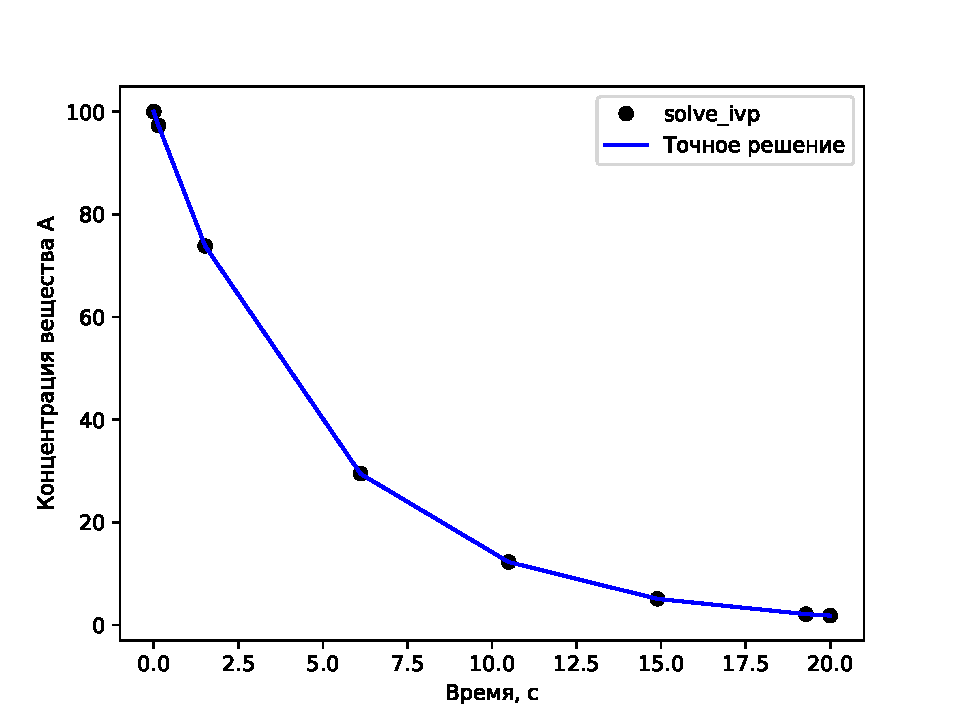
\includegraphics[width=.95\linewidth]{./pics/Figure_34}
\end{minipage}
\begin{minipage}{.5\linewidth}
	\begin{itemize}
		\item Данный подход оправдан в тех случаях, когда требуется определить только конечную концентрацию реагента, однако для отслеживания изменения концентрации во времени с более высокой дискретностью можно передать специальную последовательность точек по времени в опциональном аргументе \texttt{t\_eval}.
	\end{itemize}
\end{minipage}
\vfill
\end{frame}

\begin{frame}[fragile]{Обыкновенные дифференциальные уравнения}
\scriptsize
\begin{itemize}
	\item Разобьем наш интервал интегрирования на 21 точку по времени:

\begin{lstlisting}[language=iPython, numbers=none, frame=none]
In [3]: t0, tf = 0, 20
   ...: t_eval = np.linspace(t0, tf, 20)
   ...: solution = solve_ivp(func, (t0, tf), [y0], t_eval=t_eval)
   ...: t, y = solution.t, solution.y[0]
\end{lstlisting}

	\item В опциональный  аргумент \texttt{dense\_output} можно передать значение \textcolor{ipython_green}{\texttt{True}} для определения объекта \texttt{OdeSolution} с атрибутом \texttt{sol} как одним из возвращаемых объектов. 
	\item Данный функционал можно использовать для генерации значений решения в промежуточных точках по времени:

\begin{lstlisting}[language=iPython, numbers=none, frame=none]
# Начальная и конечные точки по времени интегрирования
t0, tf = 0, 20

# Интегрирования дифференциального уравнения
solution = solve_ivp(func, (t0, tf), [y0], dense_output=True)
t = np.linspace(t0, tf, 20)
y = solution.sol(t)[0]
\end{lstlisting}
	\item Объект \texttt{solution.sol} можно вызывать: значение независимой переменной~-- времени~-- передается в него как аргумент, и возвращается массив решений в этот момент времени. В рассмотренном случае есть только одна независимая переменная \texttt{y}, поэтому используется индекс \texttt{[0]}.
\end{itemize}
\vfil
\end{frame}

\begin{frame}[fragile]{Обыкновенные дифференциальные уравнения}
\scriptsize
\begin{minipage}{.48\linewidth}
	\centering
	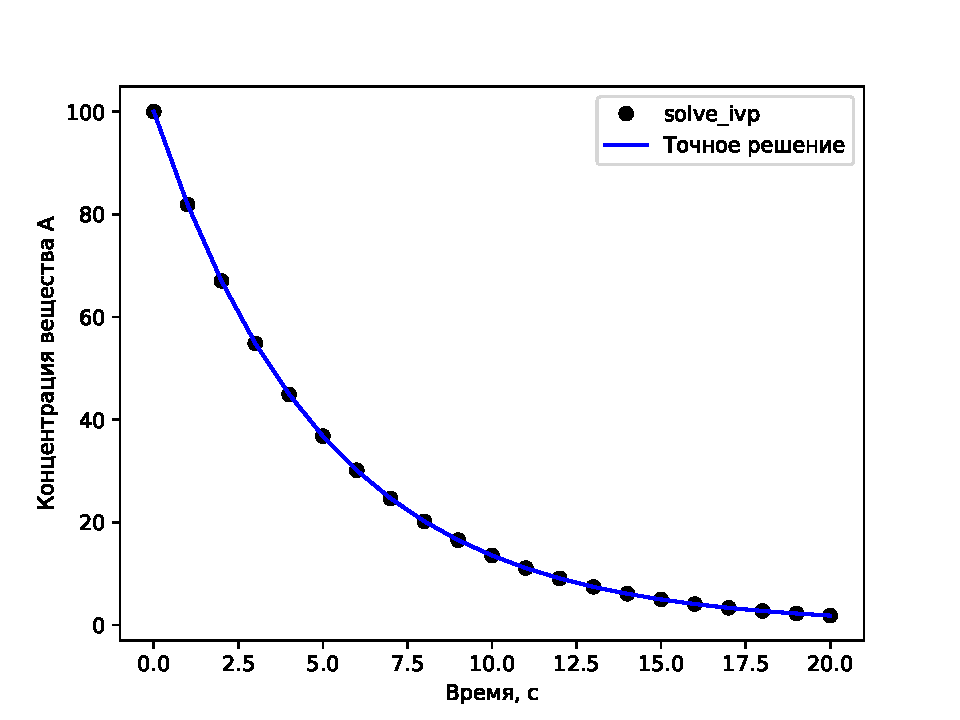
\includegraphics[width=\linewidth]{./pics/Figure_35}
\end{minipage}
\begin{minipage}{.5\linewidth}
\begin{itemize}
	\item Аналогично методу \texttt{quad}, дополнительные аргументы можно передать через параметр \texttt{args}. 
	\item В рассмотренном выше примере константа скорости реакции \texttt{k} определена в глобальной области видимости, однако лучше передавать эту переменную явным образом:
		
\begin{lstlisting}[language=iPython, numbers=none, frame=none]
def func(t, y, k):
    return -k * y
\end{lstlisting}
\end{itemize}
\end{minipage}
\begin{itemize}
	\item Дополнительные аргументы должны указываться после независимой и зависимой переменных. 
	В таком случае вызов метода \texttt{solve\_ivp} будет выглядеть следующим образом:
	
\begin{lstlisting}[language=iPython, numbers=none, frame=none]
solution = solve_ivp(func, (t0, tf), [y0], args=(k,))
\end{lstlisting}
\end{itemize}
\vfil
\end{frame}


\subsubsection{Система взаимосвязанных ОДУ первого порядка}
\begin{frame}[fragile]{Система взаимосвязанных ОДУ первого порядка}
\scriptsize
\begin{alertblock}{\footnotesize{Решение системы ОДУ первого порядка}}
	Метод \texttt{solve\_inp} также может быть использован для решения системы взаимосвязанных ОДУ первого порядка с несколькими зависимыми переменными $y_1(t), y_2(t),\dots, y_n(t)$: 
\end{alertblock}

\begin{equation*}
	\left\{
	\begin{aligned}
		\dfrac{dy_1}{dt} &= f_1\left(y_1, y_2,\dots, y_n; t\right)\\
		\dfrac{dy_2}{dt} &= f_2\left(y_1, y_2,\dots, y_n; t\right)\\
		\dots \\
		\dfrac{dy_n}{dt} &= f_n\left(y_1, y_2,\dots, y_n; t\right)
	\end{aligned}
	\right.
\end{equation*}

\begin{lstlisting}[language=iPython, numbers=none, ]
def func(t, y):
    # y = [y1, y2, ... yn] - последовательность зависимых переменных
    dy1dt = f1(y, t) 
    dy2dt = f2(y, t)
    # ... и т.д.
    # Возвращаются вычисленные производные в последовательности,
    # например, в кортеже
    return dy1dt, dy2dt, ... dyndt
\end{lstlisting}
\vfil
\end{frame}

\begin{frame}[fragile]{Система взаимосвязанных ОДУ первого порядка}
\scriptsize
Для наглядной демонстрации рассмотрим следующую схему химических реакций:

$$A \rightarrow B \rightarrow C$$

\noindent с константами скоростей $k_1$ и $k_2$. Уравнения, описывающие скорость изменения концентраций компонентов по времени, записываются следующим образом:

\begin{equation*}
	\left\{
	\begin{aligned}
		\dfrac{d\left[A\right]}{dt} &= -k_1\left[A\right] \\
		\dfrac{d\left[B\right]}{dt} &=  k_1\left[A\right] - k_2\left[B\right] \\
		\dfrac{d\left[C\right]}{dt} &=  k_2\left[B\right] \\
	\end{aligned}
	\right.
\end{equation*}


Для численного решения предположим $y_1 \equiv \left[A\right]$,  $y_2 \equiv \left[B\right]$ и $y_3 \equiv \left[C\right]$:
\begin{equation*}
	\left\{
	\begin{aligned}
		\dfrac{d\left[A\right]}{dt} &= -k_1y_1 \\
		\dfrac{d\left[B\right]}{dt} &=  k_1y_1 - k_2y_2 \\
		\dfrac{d\left[C\right]}{dt} &=  k_2y_2 \\
	\end{aligned}
	\right.
\end{equation*}
\vfil
\end{frame}

\begin{frame}[fragile]{Система взаимосвязанных ОДУ первого порядка}
\scriptsize
Зададимся значениями констант: $k_1 = 0.2 \text{ } c^{-1}$, $k_2 = 0.8 \text{ } c^{-1}$ и начальными условиями: $y_1(0) = 100$, $y_2(0) = 0$ $y_3(0) = 0$. 

\begin{lstlisting}[language=iPython, numbers=none, frame=none]
In [1]: import numpy as np
   ...: from scipy.integrate import solve_ivp

In [2]: # константы скоростей и начальные условия 
   ...: k1, k2 = 0.2, 0.8
   ...: a0, b0, c0 = 100, 0, 0
   ...: t0, tf = 0, 20

In [3]: def func(t, y, k1, k2):
   ...:     """"Returns dy_i/dt = f(t, y_i) at time t."""
   ...:     y1, y2, y3 = y
   ...:     dy1dt = -k1 * y1
   ...:     dy2dt = k1 * y1 - k2 * y2
   ...:     dy3dt = k2 * y2
   ...:
   ...:     return dy1dt, dy2dt, dy3dt
   ...:

In [4]: y0 = a0, b0, c0
\end{lstlisting}
\vfil
\end{frame}

\begin{frame}[fragile]{Система взаимосвязанных ОДУ первого порядка}
\scriptsize	
\begin{lstlisting}[language=iPython, numbers=none, frame=none]
In [5]: solution = solve_ivp(func, (t0, tf), y0,  
   ...:                      dense_output=True, args=(k1, k2))
   ...: t = np.linspace(t0, tf, 50)
   ...: a, b, c = solution.sol(t)

In [6]: # аналитическое решение
   ...: a_exact = a0 * np.exp(-k1 * t)
   ...: b_exact = a0 * k1 / (k2 - k1) * (np.exp(-k1 * t) - np.exp(-k2 * t))
   ...: c_exact = a0 - a_exact - b_exact
\end{lstlisting}
\vfill
\end{frame}

\begin{frame}[fragile]{Система взаимосвязанных ОДУ первого порядка}
\scriptsize
\begin{figure}[h!]
	\centering
	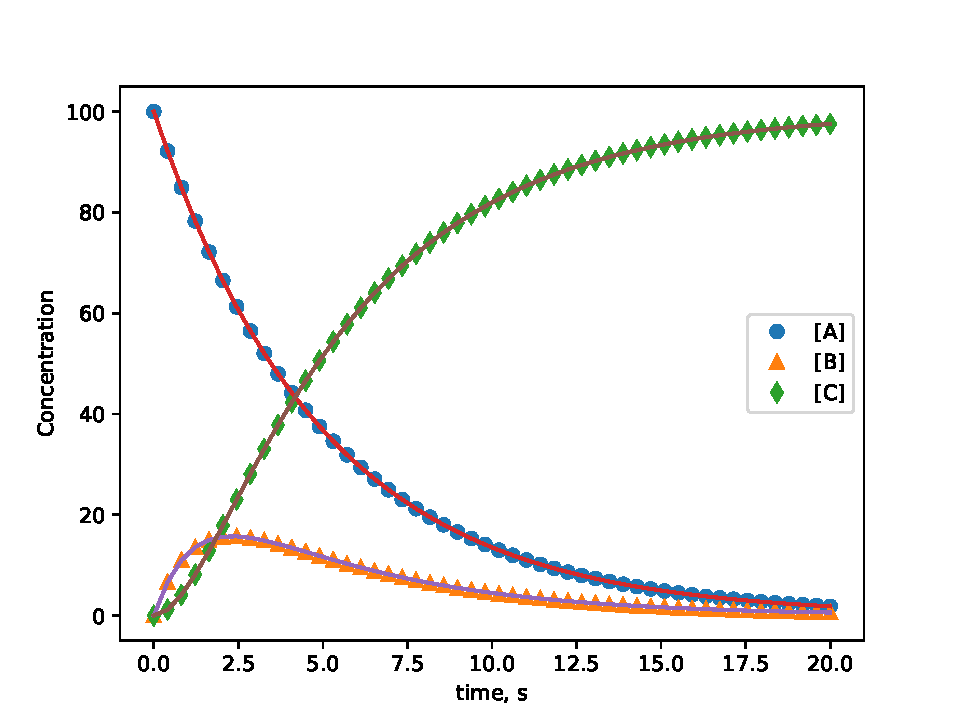
\includegraphics[width=.7\linewidth]{./pics/Figure_36}
\end{figure}
\vfil
\end{frame}


\section{Интерполяция и аппроксимация}
\sectionframe

\subsection{Одномерная интерполяция}
\begin{frame}[fragile]{Одномерная интерполяция}
\scriptsize
\begin{itemize}
	\item Метод \texttt{scipy.interpolate.interp1d} представляет метод одномерной интерполяции. 
	\item Данный метод в качестве входных параметров принимает массивы точек \texttt{x} и \texttt{y}, а возвращает объект функции, который можно вызывать для получения интерполируемых значений в промежуточных точках \texttt{x}. 
	\item По умолчанию используется линейная схема интерполяции, однако существует возможность применения и других вариантов.
\end{itemize}

\begin{table}[h!]
%	\caption{Схемы интерполяции, передаваемые в аргументе \texttt{kind} при вызове метода \texttt{scipy.interpolate.interp1d}}
%	\label{tab:interp1d}
	\begin{tabular*}{\linewidth}{p{0.15\linewidth}p{0.8\linewidth}}
		\hline
		\textbf{\texttt{kind} }& \textbf{Описание} \\
		\hline
		
		\textcolor{ipython_red}{\texttt{'linear'}} & Принятая по умолчанию линейная интерполяция, использующая при расчетах только значения из исходных данных, охватывающих требуемую точку \\
		
		\textcolor{ipython_red}{\texttt{'nearest'}} & Привязка к ближайшей	 точке данных \\
		
		\textcolor{ipython_red}{\texttt{'zero'}} & Сплайн нулевого порядка: интерполирует по последнему наблюдаемому значению при проходе по массиву данных \\
		
		\textcolor{ipython_red}{\texttt{'slinear'}} & Интерполяция сплайном первого порядка (аналог \textcolor{ipython_red}{\texttt{'linear'}}) \\
		
		\textcolor{ipython_red}{\texttt{'quadratic'}} & Интерполяция сплайном второго порядка \\
		
		\textcolor{ipython_red}{\texttt{'cubic'}} & Интерполяция кубическим сплайном \\
		
		\textcolor{ipython_red}{\texttt{'previous'}} & Используется предыдущая точка данных \\
		
		\hline
	\end{tabular*}
\end{table}
\vfil
\end{frame}

\begin{frame}[fragile]{Одномерная интерполяция}
\scriptsize
\begin{lstlisting}[language=iPython, numbers=none, frame=none ]
In [1]: import numpy as np
   ...: from scipy.interpolate import interp1d

In [2]: a, nu, k = 10, 4, 2

In [3]: def func(x, a, nu, k):
   ...:     return a * np.exp(-k * x) * np.cos(2 * np.pi * nu * x)
   ...:

In [4]: xmax, nx = 0.5, 8
   ...: x = np.linspace(0, xmax, nx)
   ...: y = func(x, a, nu, k)

In [5]: nearest = interp1d(x, y, kind='nearest')
   ...: linear = interp1d(x, y)
   ...: cubic = interp1d(x, y, kind='cubic')
\end{lstlisting}
\vfill
\end{frame}

\begin{frame}[fragile]{Одномерная интерполяция}
\scriptsize
\begin{figure}[h!]
	\centering
	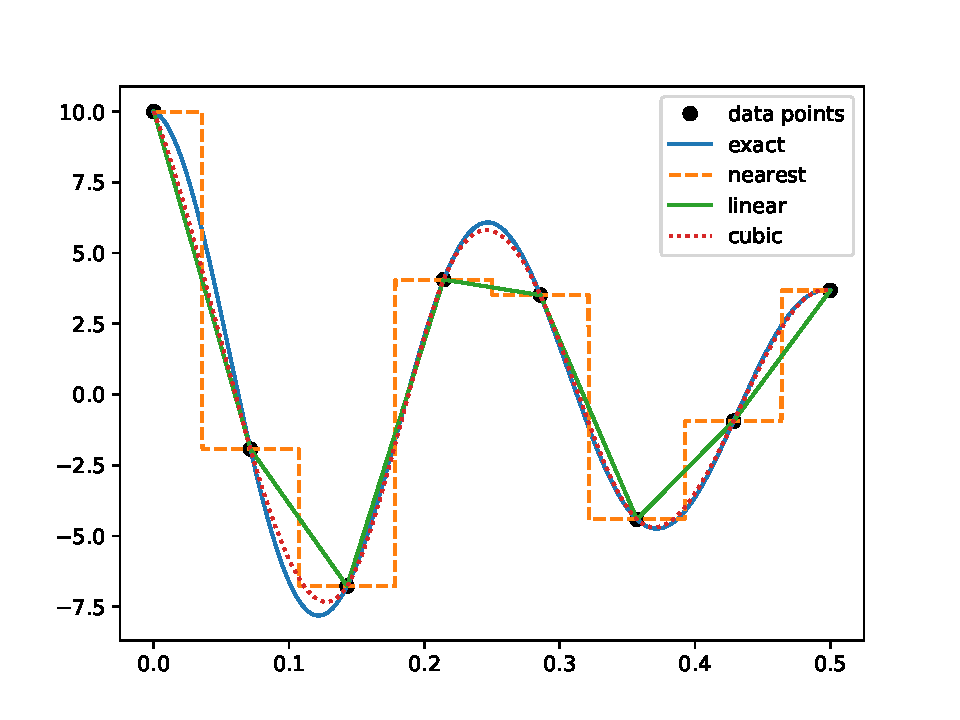
\includegraphics[width=.7\linewidth]{./pics/Figure_37}
\end{figure}
\vfil
\end{frame}


\subsection{Нелинейная аппроксимация методом \\ наименьших квадратов}
\begin{frame}[fragile]{Нелинейная аппроксимация методом \\ наименьших квадратов}
\scriptsize
В библиотеке SciPy реализована нелинейная аппроксимация методом наименьших квадратов в виде  \texttt{scipy.optimize.leastsq}. Базовая сигнатура вызова данного метода выглядит следующим образом:

\begin{lstlisting}[language=iPython, numbers=none, frame=none ]
scipy.optimize.leastsq(func, x0, args=())
\end{lstlisting}

\begin{itemize}
	\item Данный метод выполняет аппроксимацию последовательности точек данных \texttt{y} моделируемой функцией \texttt{f}, зависящей от одного или нескольких параметров аппроксимации. 
	\item В функцию \texttt{leastsq} необходимо передать соответствующий объект функции \texttt{func}, которая возвращает разность между \texttt{y} и \texttt{f} (остатки). 
	\item Также необходимо задать начальное приближение для \texttt{x0}. 
	\item Если функция \texttt{func} требует дополнительные аргументы, то их можно передать в кортеже \texttt{args}. 
	Для наглядности рассмотрим аппроксимацию искусственно зашумленной функции затухающего косинуса 
	$$ f(t) = ae^{-t/\tau}\cos2\pi\nu t $$
\end{itemize}

\vfil
\end{frame}

\begin{frame}[fragile]{Нелинейная аппроксимация методом \\ наименьших квадратов}
\scriptsize
\begin{lstlisting}[language=iPython, numbers=none,  frame=none, ]
In [1]: import numpy as np

In [2]: a, freq, tau = 10, 4, 0.5

In [3]: def f(t, a, freq, tau):
   ...:     return a * np.exp(-t / tau) * np.cos(2 * np.pi * freq * t)
   ...:

In [4]: tmax, dt = 1, 0.01

In [5]: t = np.arange(0, tmax, dt)

In [6]: y_exact = f(t, a, freq, tau)

In [7]: y = y_exact + np.random.randn(y_exact.shape[0]) * 2
\end{lstlisting}
\vfill
\end{frame}

\begin{frame}[fragile]{Нелинейная аппроксимация методом \\ наименьших квадратов}
\scriptsize
\begin{figure}[h!]
	\centering
	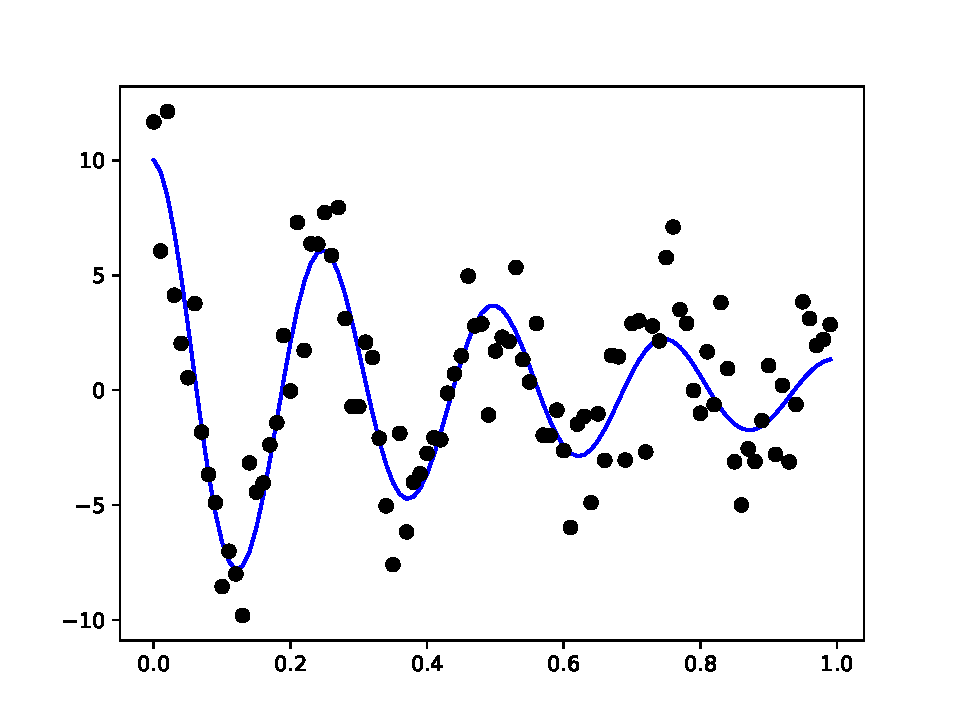
\includegraphics[width=.68\linewidth]{./pics/Figure_38}
\end{figure}
\vfil
\end{frame}

\begin{frame}[fragile]{Нелинейная аппроксимация методом \\ наименьших квадратов}
\scriptsize
Задача аппроксимации зашумленного набора данных сводится к определению параметров \texttt{a}, \texttt{freq} и \texttt{tau} (представим, что они нам неизвестны). 
\begin{itemize}
	\item Для решения этой задачи сначала необходимо определить функцию \texttt{residuals}:

\begin{lstlisting}[language=iPython, numbers=none,  frame=none, ]
In [9]: def residuals(params, y, t):
   ...:     a, freq, tau = params
   ...:     return y - f(t, a, freq, tau)
   ...:
\end{lstlisting}

	\item Первый аргумент~-- последовательность параметров \texttt{params} которые для лучшей читаемости кода распаковываются в именованные переменные. 
	\item Требуемые дополнительные аргументы: набор точек данных \texttt{y} и независимая переменная \texttt{t}. 
	\item Далее необходимо задать начальные приближения для параметров и вызвать метод \texttt{leastsq}:

\begin{lstlisting}[language=iPython, numbers=none,  frame=none, ]
In [10]: from scipy.optimize import leastsq

In [11]: params0 = 5, 5, 1

In [12]: plsq = leastsq(residuals, params0, args=(y, t))

In [13]: plsq[0]
Out[13]: array([9.1920154, 4.0158567, 0.593839 ])
\end{lstlisting}

\end{itemize}

Действительные значения параметров \texttt{a, freq, tau = 10, 4, 0.5}, таким образом, учитывая шум, добавленный к исходным данным, результат можно считать вполне приемлемым.
\vfill
\end{frame}


\begin{frame}[fragile]{Нелинейная аппроксимация методом \\ наименьших квадратов}
\scriptsize
\centering
	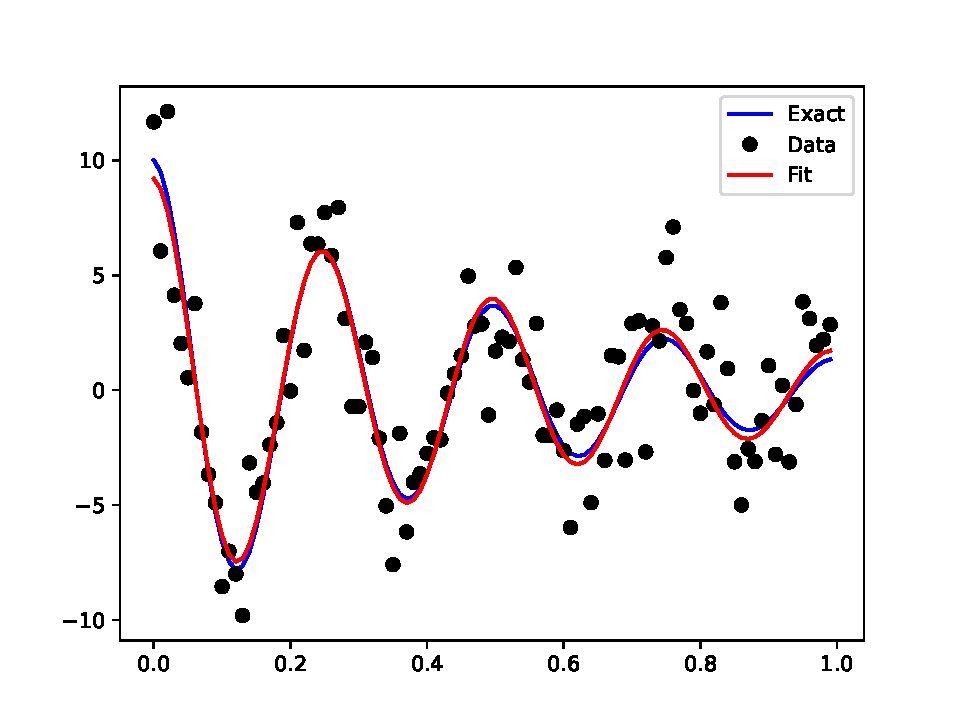
\includegraphics[width=.68\linewidth]{./pics/Figure_39}
\vfill
\end{frame}


\contactsframe[\Large \textbf{Благодарю за внимание!}]{
	
	\bigskip
	
\includegraphics[width=.05\textwidth]{pics/home} \quad Учебный корпус №2, ауд. 136 \\
	
\includegraphics[width=.05\textwidth]{pics/mail} \quad chuva@tpu.ru \\
	
\includegraphics[width=.03\textwidth]{pics/tel} \quad +7-962-782-66-15
}

\end{document}

